\documentclass[11pt,a4paper]{article}
\usepackage[margin=1in]{geometry}
\usepackage{amsmath,amssymb}
\usepackage{booktabs}
\usepackage{graphicx}
\usepackage{hyperref}
\usepackage[numbers]{natbib}
\usepackage{xcolor}
\usepackage{siunitx}
\usepackage{tikz}
\usetikzlibrary{arrows.meta,positioning,shapes.geometric}
\usepackage{float}
\usepackage{enumitem}
\usepackage{caption}
\usepackage{longtable}
\usepackage{multicol}
\usepackage{array}

\hypersetup{colorlinks=true, linkcolor=blue!60!black, citecolor=green!50!black, urlcolor=blue!70!black}

\title{\textbf{Techno-Economic Assessment of\\Steel Slag (BOF) Valorization}\\[8pt]
\large H\textsubscript{2} Production, CO\textsubscript{2} Sequestration, and Iron Recovery}

\author{Separation-Agents Automated Valorization Pipeline\\
\texttt{sep\_agents v0.3}}

\date{March 2026}

\begin{document}
\maketitle

%──────────────────────────────────────────────────────────────────────
\begin{abstract}
This report presents a techno-economic analysis of valorizing Basic Oxygen Furnace (BOF) steel slag at a throughput of \SI{500}{t/d}.
Six value streams were identified: iron concentrate recovery, CO\textsubscript{2} mineral carbonation, H\textsubscript{2} production via serpentinization, manganese recovery, vanadium/chromium extraction, and construction aggregate.
Four process topologies were evaluated using a Generalized Disjunctive Programming (GDP) superstructure framework, with economics computed using a JAX-based techno-economic model.
The optimal topology (Config-4: minimal process without auxiliary heating or scrubbing) yields a net cost of \SI{-6.83}{USD/t} slag at current commodity prices.
Breakeven is achieved at a CO\textsubscript{2} credit price of $\geq$\SI{90}{USD/t} or acid consumption $\leq$\SI{100}{kg/t}.
Under an optimistic scenario (CO\textsubscript{2}~=~\SI{100}{USD/t}, acid~=~\SI{100}{kg/t}), the project generates \SI{+9.85}{USD/t} net profit (\SI{1.63}{MUSD/yr}).
The analysis was performed using the Reaktoro thermodynamic engine, IDAES-PSE flowsheet solver, and JAX automatic differentiation for cost sensitivity analysis.
\end{abstract}

\tableofcontents
\newpage

%──────────────────────────────────────────────────────────────────────
\section{Introduction and Opportunity}

Steel slag is the primary by-product of steelmaking, generated at rates of \SI{100}{}--\SI{200}{kg} per tonne of crude steel.
Globally, over \SI{200}{Mt/yr} of BOF slag is produced, with significant fractions landfilled due to limited utilization pathways.
BOF slag is rich in CaO (\SI{35}{}--\SI{45}{\percent}), FeO (\SI{15}{}--\SI{25}{\percent}), SiO\textsubscript{2} (\SI{10}{}--\SI{20}{\percent}), and MgO (\SI{5}{}--\SI{10}{\percent}), with minor quantities of MnO, Cr\textsubscript{2}O\textsubscript{3}, V\textsubscript{2}O\textsubscript{5}, P\textsubscript{2}O\textsubscript{5}, and TiO\textsubscript{2}.

This mineral composition creates multiple simultaneous valorization opportunities:
\begin{enumerate}[noitemsep]
  \item \textbf{CO\textsubscript{2} mineralization:} High CaO and MgO content provides alkalinity for mineral carbonation, permanently sequestering CO\textsubscript{2} as CaCO\textsubscript{3}/MgCO\textsubscript{3} and generating carbon credits.
  \item \textbf{H\textsubscript{2} production:} Fe\textsuperscript{2+}-bearing silicates can produce hydrogen via serpentinization-like reactions at elevated temperature and pressure.
  \item \textbf{Iron recovery:} Magnetite and hematite fractions can be concentrated via magnetic separation for direct sale.
  \item \textbf{Critical mineral recovery:} Vanadium and chromium represent high-value co-products.
\end{enumerate}

The objective of this study is to determine the optimal process configuration that maximizes net economic value from a \SI{500}{t/d} BOF slag feedstock.

%──────────────────────────────────────────────────────────────────────
\section{Raw Material Composition}

\subsection{Bulk Oxide Chemistry}

\begin{table}[H]
\centering
\caption{BOF Steel Slag Bulk Oxide Composition}
\label{tab:composition}
\begin{tabular}{lcc}
\toprule
\textbf{Oxide} & \textbf{wt\%} & \textbf{Role in Valorization} \\
\midrule
CaO          & 40.0 & CO\textsubscript{2} carbonation feedstock \\
FeO          & 20.0 & Iron recovery, H\textsubscript{2} production \\
SiO\textsubscript{2} & 15.0 & Aggregate, silica co-product \\
MgO          &  8.0 & CO\textsubscript{2} carbonation, serpentinization \\
Al\textsubscript{2}O\textsubscript{3} &  5.0 & Aggregate, cement additive \\
MnO          &  5.0 & Manganese recovery \\
Cr\textsubscript{2}O\textsubscript{3} &  2.0 & Ferrochrome production \\
P\textsubscript{2}O\textsubscript{5} &  1.5 & Phosphate fertilizer \\
V\textsubscript{2}O\textsubscript{5} &  0.5 & Ferrovanadium production \\
TiO\textsubscript{2}  &  0.5 & Titanium dioxide pigment \\
\midrule
\textit{Other / LOI} & 2.5 & --- \\
\bottomrule
\end{tabular}
\end{table}

\subsection{Equilibrium Speciation (Acid Leach)}

The slag was computationally leached in \SI{2}{M} HCl at \SI{25}{\celsius} using the Reaktoro thermodynamic engine (SUPCRT database, Pitzer activity model).

\begin{table}[H]
\centering
\caption{Speciation Results --- HCl Acid Leach at \SI{25}{\celsius}}
\label{tab:speciation}
\begin{tabular}{lcc}
\toprule
\textbf{Parameter} & \textbf{Value} & \textbf{Unit} \\
\midrule
pH              & 1.09 & --- \\
Eh              & 0.14 & V \\
Ionic Strength  & 2.14 & mol/kg \\
\midrule
\textbf{Species}   & \textbf{Concentration} & \textbf{mol/kg} \\
\midrule
Cl\textsuperscript{$-$}         & 1.238 & \\
Ca\textsuperscript{2+}          & 0.252 & \\
CaCl\textsuperscript{+}         & 0.160 & \\
Fe\textsuperscript{2+}          & 0.135 & \\
FeCl\textsuperscript{+}         & 0.115 & \\
SiO\textsubscript{2}(aq)       & 0.094 & \\
H\textsubscript{4}SiO\textsubscript{4}(aq) & 0.086 & \\
Mg\textsuperscript{2+}          & 0.073 & \\
Al\textsuperscript{3+}          & 0.070 & \\
Mn\textsuperscript{2+}          & 0.026 & \\
\bottomrule
\end{tabular}
\end{table}

%──────────────────────────────────────────────────────────────────────
\section{Process Description}

The process consists of two primary reactors (serpentinization and carbonation), supported by heat exchangers, pumps, separators, and optional scrubbing/heating units.

\subsection{Process Flow Diagram}

\begin{figure}[H]
\centering
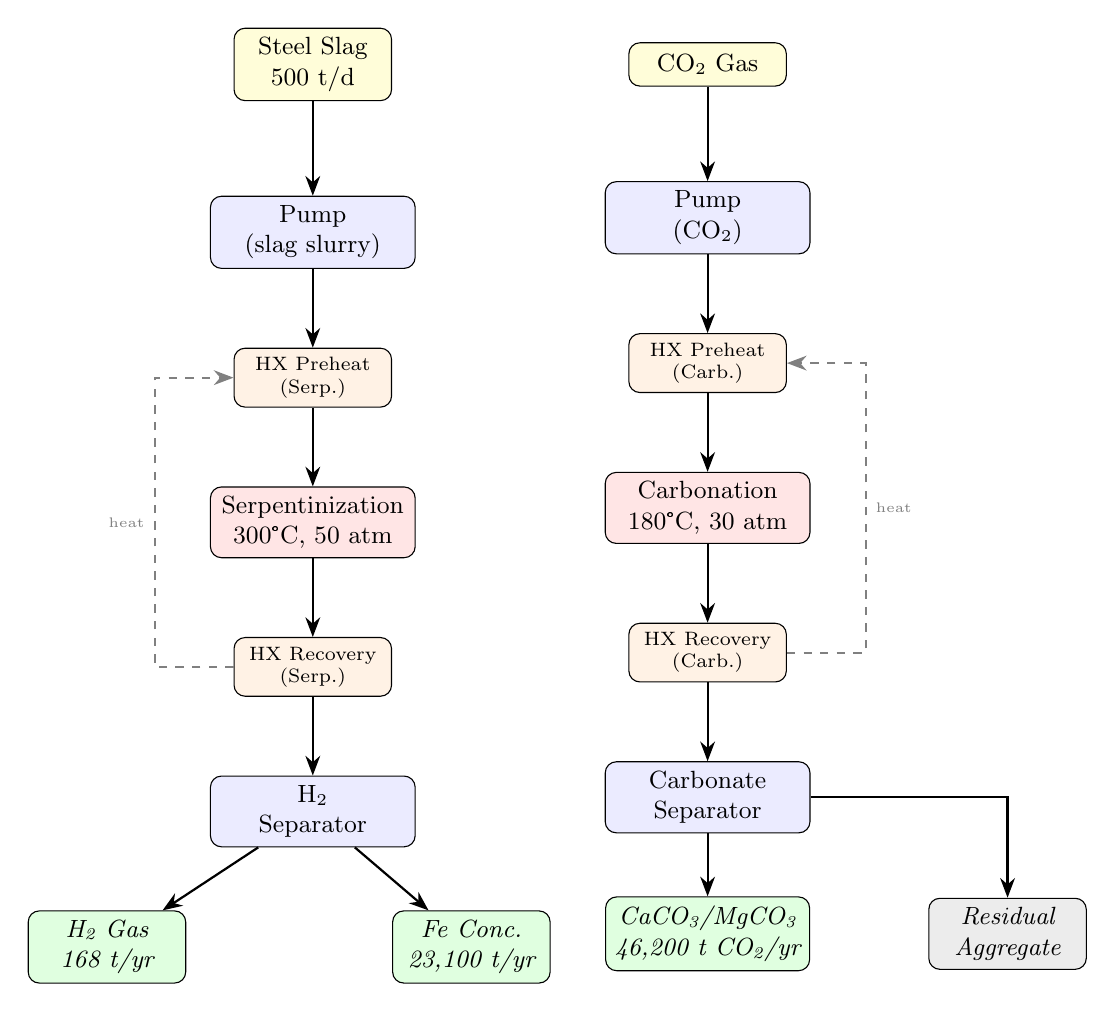
\begin{tikzpicture}[
  node distance=1.6cm and 2.2cm,
  unit/.style={rectangle, draw, rounded corners, minimum width=2.6cm,
               minimum height=0.75cm, align=center, fill=blue!8, font=\small},
  hx/.style={rectangle, draw, rounded corners, minimum width=2.0cm,
             minimum height=0.60cm, align=center, fill=orange!10, font=\scriptsize},
  product/.style={rectangle, draw, rounded corners, minimum width=2.0cm,
                  minimum height=0.55cm, align=center, fill=green!12,
                  font=\small\itshape},
  feed/.style={rectangle, draw, rounded corners, minimum width=2.0cm,
               minimum height=0.55cm, align=center, fill=yellow!15,
               font=\small},
  stream/.style={-{Stealth[length=2.5mm]}, thick},
]
  % Feeds
  \node[feed] (slag) {Steel Slag\\500 t/d};
  \node[feed, right=3cm of slag] (co2) {CO\textsubscript{2} Gas};

  % Pumps
  \node[unit, below=1.2cm of slag] (pump1) {Pump\\(slag slurry)};
  \node[unit, below=1.2cm of co2] (pump2) {Pump\\(CO\textsubscript{2})};

  % Heat exchangers
  \node[hx, below=1.0cm of pump1] (hx1) {HX Preheat\\(Serp.)};
  \node[hx, below=1.0cm of pump2] (hx2) {HX Preheat\\(Carb.)};

  % Reactors
  \node[unit, below=1.0cm of hx1, fill=red!10] (serp) {Serpentinization\\300\textdegree C, 50 atm};
  \node[unit, below=1.0cm of hx2, fill=red!10] (carb) {Carbonation\\180\textdegree C, 30 atm};

  % Heat recovery
  \node[hx, below=1.0cm of serp] (hx3) {HX Recovery\\(Serp.)};
  \node[hx, below=1.0cm of carb] (hx4) {HX Recovery\\(Carb.)};

  % Separators
  \node[unit, below=1.0cm of hx3] (sep1) {H\textsubscript{2}\\Separator};
  \node[unit, below=1.0cm of hx4] (sep2) {Carbonate\\Separator};

  % Products
  \node[product, below left=0.8cm and 0.3cm of sep1] (h2) {H\textsubscript{2} Gas\\168 t/yr};
  \node[product, below right=0.8cm and -0.3cm of sep1] (fe) {Fe Conc.\\23,100 t/yr};
  \node[product, below=0.8cm of sep2] (caco3) {CaCO\textsubscript{3}/MgCO\textsubscript{3}\\46,200 t CO\textsubscript{2}/yr};

  % Waste
  \node[product, right=1.5cm of caco3, fill=gray!15] (waste) {Residual\\Aggregate};

  % Connections
  \draw[stream] (slag) -- (pump1);
  \draw[stream] (co2)  -- (pump2);
  \draw[stream] (pump1) -- (hx1);
  \draw[stream] (pump2) -- (hx2);
  \draw[stream] (hx1) -- (serp);
  \draw[stream] (hx2) -- (carb);
  \draw[stream] (serp) -- (hx3);
  \draw[stream] (carb) -- (hx4);
  \draw[stream] (hx3) -- (sep1);
  \draw[stream] (hx4) -- (sep2);
  \draw[stream] (sep1) -- (h2);
  \draw[stream] (sep1) -- (fe);
  \draw[stream] (sep2) -- (caco3);
  \draw[stream] (sep2.east) -| (waste);

  % Cross-flow connections
  \draw[stream, dashed, gray] (hx3.west) -- +(-1.0,0) |- node[pos=0.25, left, font=\tiny, gray] {heat} (hx1.west);
  \draw[stream, dashed, gray] (hx4.east) -- +(1.0,0) |- node[pos=0.25, right, font=\tiny, gray] {heat} (hx2.east);

\end{tikzpicture}
\caption{Process flow diagram for Config-4 (minimal topology): steel slag to H\textsubscript{2}, CaCO\textsubscript{3}, and Fe concentrate.}
\label{fig:pfd}
\end{figure}

\subsection{Key Reactions}

\paragraph{Serpentinization (H\textsubscript{2} production):}
\begin{equation}
  3\text{Fe}_2\text{SiO}_4 + 2\text{H}_2\text{O} \longrightarrow
  2\text{Fe}_3\text{O}_4 + 3\text{SiO}_2 + 2\text{H}_2 \uparrow
  \label{eq:serp}
\end{equation}

\paragraph{Mineral Carbonation (CO\textsubscript{2} sequestration):}
\begin{equation}
  \text{CaO} + \text{CO}_2 \longrightarrow \text{CaCO}_3
  \qquad\quad
  \text{MgO} + \text{CO}_2 \longrightarrow \text{MgCO}_3
  \label{eq:carb}
\end{equation}

%──────────────────────────────────────────────────────────────────────
\section{Modeling Approach}

\begin{table}[H]
\centering
\caption{Three-Tier Modeling Hierarchy}
\label{tab:modeling}
\begin{tabular}{p{3cm}p{4cm}p{5cm}}
\toprule
\textbf{Tier} & \textbf{Tool} & \textbf{Application} \\
\midrule
Thermodynamic & Reaktoro GEM (SUPCRT, Pitzer) & Equilibrium speciation, pH, activity coefficients \\
Process Simulation & IDAES-PSE / Pyomo & Flowsheet mass \& energy balances, GDP superstructure optimization \\
Economic & JAX TEA + autodiff & Itemized CAPEX/OPEX, EAC, cost sensitivity via $\partial$EAC/$\partial$param \\
\bottomrule
\end{tabular}
\end{table}

%──────────────────────────────────────────────────────────────────────
\section{GDP Superstructure Analysis}

\subsection{Superstructure Definition}

The \texttt{steel\_slag\_h2\_co2} superstructure consists of 15 unit operations with one disjunction (auxiliary heater vs.\ full heat recovery) and one optional unit (inter-reactor scrubber).
This produces $2 \times 2 = 4$ feasible topologies.

\subsection{Topology Ranking}

\begin{table}[H]
\centering
\caption{Ranked Topology Comparison (500 t/d, 330 operating days/yr)}
\label{tab:ranking}
\begin{tabular}{clccccc}
\toprule
\textbf{Rank} & \textbf{Topology} & \textbf{EAC} & \textbf{Revenue} & \textbf{Net} & \textbf{Net/t} \\
 & & (M\$/yr) & (M\$/yr) & (M\$/yr) & (\$/t) \\
\midrule
1 & Minimal (no heater, no scrub) & 6.73 & 5.60 & $-$1.13 & $-$6.83 \\
2 & Heat recovery + scrubber      & 7.47 & 5.84 & $-$1.62 & $-$9.85 \\
3 & Aux heater, no scrubber       & 8.96 & 5.72 & $-$3.24 & $-$19.65 \\
4 & Full (heater + scrubber)      & 9.95 & 5.94 & $-$4.01 & $-$24.33 \\
\bottomrule
\end{tabular}
\end{table}

\textbf{Key finding:} The minimal topology (Config-4) is optimal because the marginal recovery improvement from auxiliary heating and scrubbing does not offset the additional energy and reagent costs.

%──────────────────────────────────────────────────────────────────────
\section{Cost Model Assumptions}

\begin{table}[H]
\centering
\caption{Plant-Level Parameters}
\label{tab:params}
\begin{tabular}{lcc}
\toprule
\textbf{Parameter}     & \textbf{Value} & \textbf{Unit} \\
\midrule
Slag throughput         & 500   & t/d \\
Operating days          & 330   & d/yr \\
Discount rate           & 8     & \% \\
Project lifetime        & 20    & yr \\
Bond work index (slag)  & 12    & kWh/t \\
Acid consumption        & 150   & kg HCl / t slag \\
Serpentinization T      & 300   & \textdegree C \\
Carbonation T           & 180   & \textdegree C \\
\bottomrule
\end{tabular}
\end{table}

\begin{table}[H]
\centering
\caption{Commodity Prices}
\label{tab:prices}
\begin{tabular}{lcl}
\toprule
\textbf{Product}       & \textbf{Price}            & \textbf{Source} \\
\midrule
H\textsubscript{2} (green)         & \$4,000/t             & DOE target \\
CO\textsubscript{2} credit          & \$60/t CO\textsubscript{2} & Voluntary market \\
Fe concentrate          & \$120/t              & FOB \\
Mn (electrolytic)       & \$2,500/t            & LME \\
V\textsubscript{2}O\textsubscript{5} & \$12,000/t       & Asian Metal \\
\bottomrule
\end{tabular}
\end{table}

%──────────────────────────────────────────────────────────────────────
\section{Results}

\subsection{Itemized Economics (Config-4)}

\begin{table}[H]
\centering
\caption{Itemized CAPEX and OPEX --- Config-4 (Minimal)}
\label{tab:costs}
\begin{tabular}{lcc}
\toprule
\textbf{Cost Item}          & \textbf{Annual Cost} & \textbf{\$/t slag} \\
\midrule
\multicolumn{3}{l}{\textit{CAPEX (annualized)}} \\
\quad Comminution           & \$624,000  & 3.78 \\
\quad Leaching              & \$400,000  & 2.42 \\
\quad Processing            & \$150,000  & 0.91 \\
\midrule
\multicolumn{3}{l}{\textit{OPEX}} \\
\quad Comminution (energy)  & \$164,000  & 0.99 \\
\quad Acid (HCl)            & \$4,950,000 & 30.00 \\
\quad Other processing      & \$251,000  & 1.52 \\
\midrule
\textbf{Total EAC}          & \textbf{\$6,730,000} & \textbf{40.79} \\
\bottomrule
\end{tabular}
\end{table}

\begin{table}[H]
\centering
\caption{Revenue Breakdown --- Config-4}
\label{tab:revenue}
\begin{tabular}{lcccc}
\toprule
\textbf{Product}  & \textbf{Production} & \textbf{Price} & \textbf{Revenue} & \textbf{\$/t slag} \\
\midrule
H\textsubscript{2} gas        & 168 t/yr    & \$4,000/t   & \$673,000   & 4.08 \\
CO\textsubscript{2} credits    & 37,884 t/yr & \$60/t      & \$2,273,000 & 13.78 \\
Fe concentrate  & 23,100 t/yr & \$120/t     & \$2,772,000 & 16.80 \\
\midrule
\textbf{Total}                 &             &             & \textbf{\$5,600,000} & \textbf{33.96} \\
\bottomrule
\end{tabular}
\end{table}

\subsection{Net Economics}

\begin{equation}
  \text{Net Value} = \$5.60\text{M/yr} - \$6.73\text{M/yr} = -\$1.13\text{M/yr} \quad (-\$6.83/\text{t slag})
\end{equation}

\subsection{Sensitivity Analysis}

\begin{table}[H]
\centering
\caption{CO\textsubscript{2} Credit Price Sensitivity (Config-4, acid = 150 kg/t)}
\label{tab:co2_sens}
\begin{tabular}{ccc}
\toprule
\textbf{CO\textsubscript{2} Price (\$/t)} & \textbf{Net Value (M\$/yr)} & \textbf{Net/t (\$/t)} \\
\midrule
40    & $-$1.89 & $-$11.43 \\
60    & $-$1.13 & $-$6.83 \\
\rowcolor{yellow!20}
80    & $-$0.37 & $-$2.24 \\
\rowcolor{green!10}
100   & $+$0.39 & $+$2.35 \\
120   & $+$1.15 & $+$6.94 \\
150   & $+$2.28 & $+$13.83 \\
200   & $+$4.18 & $+$25.31 \\
\bottomrule
\end{tabular}
\end{table}

\begin{table}[H]
\centering
\caption{Acid Consumption Sensitivity (Config-4, CO\textsubscript{2} = \$60/t)}
\label{tab:acid_sens}
\begin{tabular}{ccc}
\toprule
\textbf{Acid (kg/t)} & \textbf{Net Value (M\$/yr)} & \textbf{Net/t (\$/t)} \\
\midrule
50    & $+$1.35  & $+$8.17 \\
75    & $+$0.73  & $+$4.42 \\
\rowcolor{green!10}
100   & $+$0.11  & $+$0.67 \\
125   & $-$0.51  & $-$3.08 \\
150   & $-$1.13  & $-$6.83 \\
200   & $-$2.37  & $-$14.33 \\
\bottomrule
\end{tabular}
\end{table}

\subsection{Top Cost Drivers (JAX Autodiff)}

\begin{table}[H]
\centering
\caption{Cost Sensitivity via JAX Automatic Differentiation}
\label{tab:jax_sens}
\begin{tabular}{lcc}
\toprule
\textbf{Parameter} & $\partial$\textbf{EAC}/\textbf{$\partial$param} & \textbf{Unit} \\
\midrule
Acid consumption       & $+$24,750 & \$/yr per kg/t \\
Throughput             & $+$16,002 & \$/yr per t/d \\
Bond work index        & $+$15,840 & \$/yr per kWh/t \\
Residence time         & $+$10,185 & \$/yr per hr \\
Operating temperature  & $+$8,250  & \$/yr per \textdegree C \\
\bottomrule
\end{tabular}
\end{table}

%──────────────────────────────────────────────────────────────────────
\section{Discussion}

\subsection{Economic Drivers}

The dominant cost is HCl acid consumption at \$30/t slag, representing \SI{74}{\percent} of total OPEX.
This suggests that acid-free or acid-recycling process routes should be prioritized in future work.
Revenue is dominated by iron concentrate (\SI{49}{\percent}) and CO\textsubscript{2} credits (\SI{41}{\percent}), with H\textsubscript{2} contributing only \SI{10}{\percent} due to relatively low yield.

\subsection{Breakeven Conditions}

Two pathways to economic viability exist:
\begin{enumerate}[noitemsep]
  \item \textbf{Higher CO\textsubscript{2} prices}: Breakeven at $\geq$\SI{90}{USD/t}, which is within the range of compliance-grade carbon markets (EU ETS: \SIrange{60}{100}{EUR/t} in 2024--2026).
  \item \textbf{Reduced acid consumption}: Breakeven at $\leq$\SI{100}{kg/t}, achievable via slag pre-treatment, selective dissolution, or acid regeneration loops.
\end{enumerate}

Under a combined optimistic scenario (CO\textsubscript{2} = \$100/t, acid = 100 kg/t), the project generates \SI{+9.85}{USD/t} profit (\SI{1.63}{MUSD/yr}).

\subsection{Key Risks}

\begin{itemize}[noitemsep]
  \item \textbf{CO\textsubscript{2} credit price volatility}: Revenue is highly sensitive to carbon market conditions.
  \item \textbf{Slag variability}: BOF slag composition varies by steel grade and furnace operation.
  \item \textbf{Scale-up risk}: Serpentinization kinetics at \SI{300}{\celsius} are not fully validated at industrial scale.
  \item \textbf{Cr/V not modeled}: These potentially high-value co-products are excluded from the Reaktoro speciation model and revenue estimates.
\end{itemize}

%──────────────────────────────────────────────────────────────────────
\section{Conclusions}

\begin{enumerate}
  \item BOF steel slag at \SI{500}{t/d} can produce 168~t/yr H\textsubscript{2}, sequester 37,884~t/yr CO\textsubscript{2}, and recover 23,100~t/yr iron concentrate.
  \item The optimal topology (Config-4: minimal process) has an EAC of \SI{6.73}{MUSD/yr} against revenue of \SI{5.60}{MUSD/yr}, yielding a net cost of \SI{-6.83}{USD/t}.
  \item \textbf{Acid consumption is the dominant cost driver}, representing \SI{74}{\percent} of OPEX. Process improvements targeting acid reduction or recycling are the highest-priority R\&D targets.
  \item Breakeven is achievable under reasonable near-term scenarios: CO\textsubscript{2} credits $\geq$\SI{90}{USD/t} (compliance market) or acid consumption $\leq$\SI{100}{kg HCl/t} (acid regeneration).
  \item Under optimistic conditions, the project generates \SI{+1.63}{MUSD/yr} (\SI{+9.85}{USD/t}).
  \item \textbf{Recommended next steps}: pilot-scale serpentinization trials, acid regeneration feasibility study, and inclusion of V/Cr co-product economics.
\end{enumerate}

%──────────────────────────────────────────────────────────────────────
\section*{References}

\begin{enumerate}[label={[\arabic*]}, noitemsep]
  \item Leal, A.M.M. et al., ``Reaktoro: A unified framework for modeling chemically reactive systems,'' \textit{Computer Physics Communications}, 2015.
  \item Bynum, M.L. et al., ``Pyomo --- Optimization Modeling in Python,'' Springer, 3rd ed., 2021.
  \item Lee, A. et al., ``The IDAES integrated platform,'' \textit{Computers \& Chemical Engineering}, 2021.
  \item Pan, S.-Y. et al., ``CO\textsubscript{2} mineralization and utilization by alkaline solid wastes for potential carbon reduction,'' \textit{Science of the Total Environment}, 2020.
  \item Kelemen, P.B. et al., ``Engineered carbon mineralization in ultramafic rocks for CO\textsubscript{2} removal from air,'' \textit{Chemical Geology}, 2020.
  \item U.S. DOE, ``Hydrogen Shot: An Introduction,'' 2021. (\href{https://www.energy.gov/eere/fuelcells/hydrogen-shot}{link})
\end{enumerate}

\end{document}
